\section{Software}
\begin{frame}{Software}
    Our project is \stress{openly} and \stress{actively} developed on
    \vcenteredinclude{\includegraphics[height=2ex]{figures/software_logos/octocat.pdf}\hspace{-0.05cm}
    
\includegraphics[height=2ex]{figures/software_logos/github.pdf}}\\
    {\color{purple}\url{https://github.com/RD-clustering/B_decays_clustering}}
    
    \bigskip
    Implemented in \vcenteredinclude{\includegraphics[height=3ex]{figures/software_logos/python.pdf}} using
    \begin{itemize}
        \item \vcenteredinclude{\includegraphics[height=4ex]{figures/software_logos/numpy_noname.pdf}} \texttt{numpy} {\footnotesize(fast numeric operations on arrays)}
        \item \vcenteredinclude{
\includegraphics[height=3.5ex]{figures/software_logos/pandas_noname.pdf}} \texttt{pandas} {\footnotesize(dataframes)}
        \item \vcenteredinclude{\includegraphics[height=4ex]{figures/software_logos/matplotlib.pdf}} \texttt{matplotlib} {\footnotesize(beautiful plots)}
        \item \vcenteredinclude{\includegraphics[height=3.5ex]{figures/software_logos/sklearn.pdf}} \texttt{scikit-learn} {\footnotesize(clustering tools)}
        \item \vcenteredinclude{\includegraphics[height=3.5ex]{figures/software_logos/scipy.pdf}} \texttt{scipy} {\footnotesize(integration and clustering tools)}
        \item \vcenteredinclude{\includegraphics[height=3.5ex]{figures/software_logos/jupyter.pdf}} \texttt{jupyter} {\footnotesize(interactive notebooks)}
        \item \vcenteredinclude{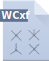
\includegraphics[height=3ex]{figures/software_logos/wcxf.pdf}} \texttt{wcxf} {\footnotesize(specify Wilson coefficients in a variety of bases)}
        \item \vcenteredinclude{\includegraphics[height=3ex]{figures/software_logos/wilson.pdf}} \texttt{Wilson} {\footnotesize(running of Wilson coefficients)}
        \item \vcenteredinclude{\includegraphics[height=3ex]{figures/software_logos/flavio.pdf}} \texttt{Flavio} {\footnotesize(various observables with NP predictions)}
    \end{itemize}
\end{frame}

\begin{frame}{Software}
    \begin{itemize}
        \item Up to date documentation on read the docs:\\[3ex]
        \begin{center}\includegraphics[width=0.8\linewidth]{figures/scrot/readthedocs.png}\end{center}
        \vspace{2ex}
        \item Interactive tutorials using \vcenteredinclude{\includegraphics[height=3.5ex]{figures/software_logos/jupyter.pdf}} \texttt{jupyter notebooks}
        %\includegraphics[width=3cm]{figures/scrot/jupyter.png}
    \end{itemize}
    
    \bigskip
    
\end{frame}

\begin{frame}{Software}
    General steps:
    \begin{enumerate}
        \item \stress{Scan}: Calculate binned distributions for your observable, e.g. $\dd\Gamma/\dd q^2$
        \begin{itemize}
            \item An arbitrary python function can be specified
            \item E.g. simply take an observable from \texttt{flavio}
            \item Parallel processing supported
        \end{itemize}
        \item (optional) \stress{Add errors}: Easy interface to add various kinds of errors {\footnotesize(Poisson, flat relative errors, errors given by covariance matrix, maximally correlated errors etc.)}
        \item \stress{Cluster}: Take the binned distributions and cluster them\\
        {\footnotesize Clustering class is subclassed to support any clustering algorithm}
        \item \stress{Benchmark point}: Select one representative for each cluster
        \item \stress{Plot}: Various plotting methods are provided
    \end{enumerate}
\end{frame}

\begin{frame}[fragile]{Software}{Quick tutorial}
    Generate a sample of kinematic distributions (here $\dd\Gamma/\dd q^2$ for $\bdstaunu$) using the \mintinline{python}{Scanner} class:
    
    \begin{minted}[
        mathescape,
        linenos,
        numbersep=5pt,
        gobble=8,
        frame=lines,
        fontsize=\small,
        framesep=2mm,
        tabsize=4
    ]{python}
    
        s = Scanner()
        s.set_dfunction(
            bdlnu.dGq2,
            binning=np.linspace(bdlnu.q2min, bdlnu.q2max, 10),
            normalize=True
        )
        s.set_wpoints_equidist(
            {
                "CVL_bctaunutau": (-0.3, 0.3, 10),
                "CSL_bctaunutau": (-0.3, 0.3, 10),
                "CT_bctaunutau": (-0.4, 0.4, 10)
            },
            scale=5,
            eft='WET',
            basis='flavio'
        )
        s.run()
        s.write("output/scan", "tutorial")
    \end{minted}

\end{frame}

\begin{frame}[fragile]{Software}{Quick tutorial}
    Now we cluster it: 
    
    \begin{minted}[
    mathescape,
    linenos,
    numbersep=5pt,
    gobble=8,
    frame=lines,
    fontsize=\small,
    framesep=2mm,
    tabsize=4
    ]{python}
        c = HierarchyCluster("output/scan", "tutorial")
        c.build_hierarchy()
        c.cluster(max_d=0.1)
    \end{minted}
    
    \begin{columns}
        \column{0.4\linewidth}
        And can directly plot it:
        
        \begin{changemargin}{0.32cm}{0cm}
        \begin{minted}[
        mathescape,
        linenos,
        numbersep=5pt,
        gobble=12,
        frame=lines,
        fontsize=\small,
        framesep=2mm,
        tabsize=4
        ]{python}
            cp = ClusterPlot(df)
            cp.scatter([
                'CVL_bctaunutau',
                'CSL_bctaunutau',
                'CT_bctaunutau'
            ])
        \end{minted}
        \end{changemargin}
        \column{0.6\linewidth}
        \centering
        \includegraphics[width=5.5cm]{figures/plots/3d.pdf}
    \end{columns}
\end{frame}


\begin{frame}[fragile, t]{Software}{Quick tutorial}
\vspace{0.75cm}
\begin{minted}[
mathescape,
linenos,
numbersep=5pt,
gobble=4,
frame=lines,
fontsize=\small,
framesep=2mm,
tabsize=4
]{python}
   cp.scatter(['CVL_bctaunutau', 'CSL_bctaunutau'])
\end{minted}
\vspace{0.2cm}
\centering
\includegraphics[width=10.5cm]{figures/plots/2dpoints.pdf}
\end{frame}

\begin{frame}[fragile, t]{Software}{Quick tutorial}
\vspace{0.75cm}
\begin{minted}[
mathescape,
linenos,
numbersep=5pt,
gobble=4,
frame=lines,
fontsize=\small,
framesep=2mm,
tabsize=4
]{python}
   cp.fill(['CVL_bctaunutau', 'CSL_bctaunutau'])
\end{minted}
\centering
\includegraphics[trim=3cm 0 11cm 0, clip, width=10.5cm]{figures/plots/2dfill.pdf}
\end{frame}
